% ============================================================ quasi-closed-shell (non-aufbau) radicals
\section{Quasi-closed shells}

\begin{frame}{SOMO below HOMO (Figure 10)}
  \begin{columns}[c]
    \column{0.45\textwidth}
    \centering
    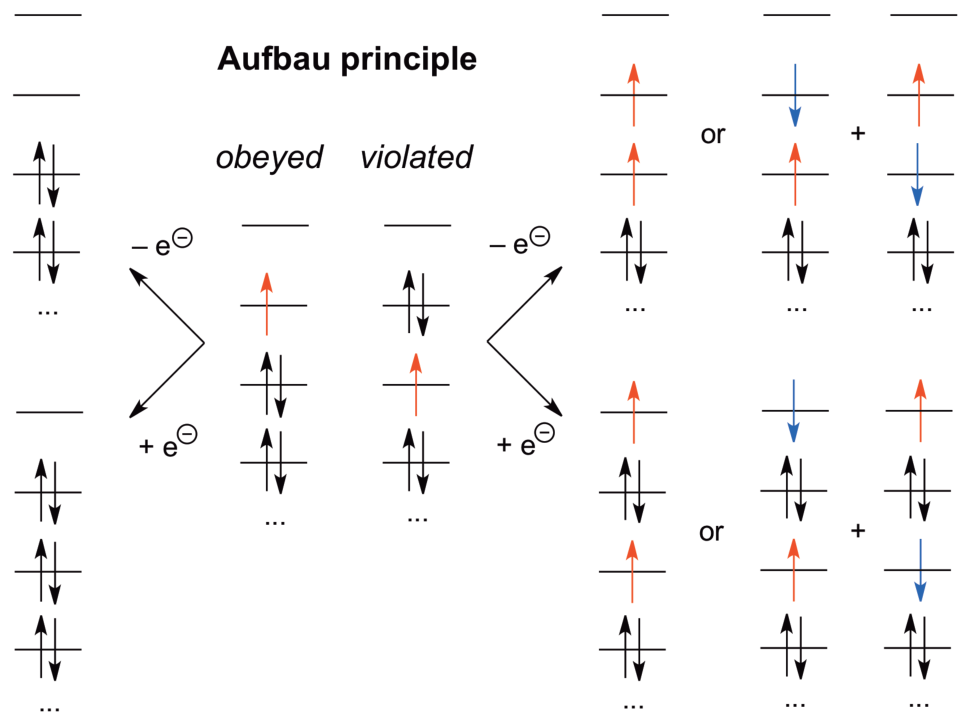
\includegraphics[width=\linewidth]{fig10_aufbau_vs_non_aufbau.png}
    \column{0.52\textwidth}
    \begin{paperclaim}
      ``upon ionization an electron is removed from the higher energy doubly occupied MO, leaving another unpaired
      electron behind, while upon addition new electron enters the former LUMO; essentially, SOMO does not participate
      in these processes.'' (p.\ 449)
    \end{paperclaim}
    \onslide<2->{\small the fingerprint is \cgold{redox}: products are \cgold{diradicals}, not closed shells}
  \end{columns}
\end{frame}

\begin{frame}{UHF orbital energies of $s^1h^2$ (1/2)}
  \begin{assume}
    frozen orbitals; SOMO $s$ ($\alpha$ only), doubly occupied $h$; core absorbed into $h_s,h_h$;
    $\varepsilon_k=E_N-E_{N-1}^{(k)}$ (Koopmans)
  \end{assume}
  configuration: \ $s\alpha,\ h\alpha,\ h\beta$ \quad pairs: $(s\alpha,h\alpha)$ same spin, $(s\alpha,h\beta)$, $(h\alpha,h\beta)$
  {\large
  \begin{align*}
    \uncover<2->{E_N}&\uncover<2->{=h_s+2h_h+\underbrace{(J_{hs}-K_{hs})}_{s\alpha,h\alpha}+\underbrace{J_{hs}}_{s\alpha,h\beta}+\underbrace{J_{hh}}_{h\alpha,h\beta}}\\
    \uncover<3->{\varepsilon_h^\alpha=E_N-E(s\alpha,h\beta)}&\uncover<3->{=h_h+J_{hh}+J_{hs}-K_{hs}}\\
    \uncover<4->{\varepsilon_h^\beta=E_N-E(s\alpha,h\alpha)}&\uncover<4->{=h_h+J_{hh}+J_{hs}}
  \end{align*}}
\end{frame}

\begin{frame}{UHF orbital energies of $s^1h^2$ (2/2)}
  {\begin{align*}
    \varepsilon_s^\alpha=E_N-E(h\alpha,h\beta)&=h_s+2J_{hs}-K_{hs}\\
    \uncover<2->{\varepsilon_s^\beta\ (\text{empty; add }s\beta)}&\uncover<2->{=h_s+J_{ss}+2J_{hs}-K_{hs}}
  \end{align*}}
  \begin{columns}[c]
    \column{0.52\textwidth}
    \onslide<3->{
    \begin{keyresult}[Scheme 3, derived]
      $\varepsilon_h^\beta-\varepsilon_h^\alpha=K_{hs}\ge0$: the donor's $\alpha$ HOMO is pulled down by exchange with the
      unpaired electron; its $\beta$ HOMO is not
    \end{keyresult}}
    \onslide<4->{\footnotesize\tick\ \cmuted{T2: all four checked against determinant energies}}
    \column{0.44\textwidth}
    \centering
    \onslide<3->{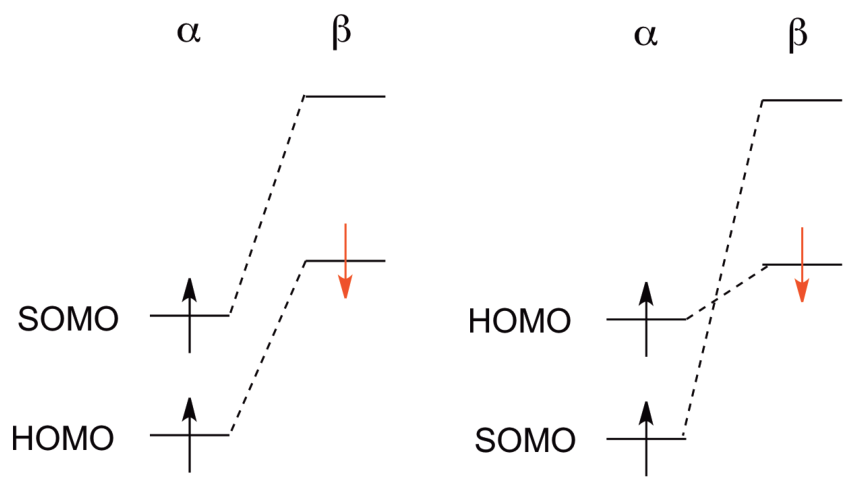
\includegraphics[width=0.78\linewidth]{scheme03_donor_HOMO_spin_polarization.png}}
  \end{columns}
\end{frame}

\begin{frame}{When does the SOMO drop below the HOMO?}
  compare within the $\alpha$ manifold:
  {\large
  \begin{align*}
    \varepsilon_s^\alpha<\varepsilon_h^\alpha
      &\iff h_s+2J_{hs}\canc<2->{-K_{hs}}<h_h+J_{hh}+J_{hs}\canc<2->{-K_{hs}}\\
      &\uncover<3->{\iff h_s+J_{hs}<h_h+J_{hh}}
  \end{align*}}
  \onslide<4->{\small radical orbital: its energy plus repulsion with \emph{one} $h$ electron, vs.\ $h$'s energy plus its \emph{self}-repulsion}
  \vskip0.3cm
  \begin{columns}[T]
    \column{0.48\textwidth}
    \onslide<5->{\begin{plainpanel}\cgold{favours conversion}: a stable radical (low $h_s$) beside an electron-rich, e.g.\ anionic,
      fragment (high $h_h$)\end{plainpanel}}
    \column{0.48\textwidth}
    \onslide<6->{\begin{paperclaim}``spatially separated stable radical center and molecular fragment serving as a source of
      high-energy doubly occupied orbitals'' (p.\ 454)\end{paperclaim}}
  \end{columns}
\end{frame}

\begin{frame}{The redox fingerprint, derived}
  \begin{columns}[T]
    \column{0.5\textwidth}
    \cgold{oxidation}
    \begin{itemize}
      \item Koopmans: $\mathrm{IP}(h)=-\varepsilon_h<\mathrm{IP}(s)$
      \item<2-> product $s^1h^1$: a diradical
      \item<3-> its states: $E_{\OSS}-E_T=2K_{sh}>0$
      \item<4-> \cgold{triplet} cation diradicals with nondegenerate SOMOs, as observed
    \end{itemize}
    \column{0.47\textwidth}
    \onslide<5->{\cgold{reduction}}
    \begin{itemize}
      \item<5-> into $s\beta$ at $\varepsilon_s^\beta$, or into $l$ at $\varepsilon_l$
      \item<6-> diradical $s^1h^2l^1$ iff $\varepsilon_l<h_s+J_{ss}+2J_{hs}-K_{hs}$
      \item<7-> \crose{a separate condition}: SOMO--HOMO conversion alone does not imply it
    \end{itemize}
    \onslide<8->{\small\cmuted{the large on-site $J_{ss}$ is what pushes $\varepsilon_s^\beta$ up}}
  \end{columns}
\end{frame}

\begin{frame}{ROHF: are these orbital energies even real?}
  \begin{paperclaim}
    ``erroneous non-aufbau occupations can be observed with restricted open-shell methods depending on the
    canonicalization parameters of the $\alpha$ and $\beta$ electrons in Fock matrix'' (p.\ 449)
  \end{paperclaim}
  spaces: core $c$ (doubly), open $o$ ($\alpha$), virtual $v$; \quad $\mathbf D^\alpha=\mathbf D_c+\mathbf D_o$, \ $\mathbf D^\beta=\mathbf D_c$
  {\large
  \[
    \uncover<2->{\delta E=\operatorname{tr}(\mathbf F^\alpha\delta\mathbf D^\alpha)+\operatorname{tr}(\mathbf F^\beta\delta\mathbf D^\beta),\qquad
    \text{rotation }p\leftrightarrow q:\ \delta\mathbf D^\sigma=\kappa(\ket p\bra q+\ket q\bra p)}
  \]}
  \onslide<3->{\small\cmuted{a rotation changes $\mathbf D^\sigma$ only if exactly one of $p,q$ is occupied in spin $\sigma$}}
\end{frame}

\begin{frame}{ROHF stationarity, rotation by rotation}
  \centering
  \renewcommand{\arraystretch}{1.3}
  \begin{tabular}{llll}
    \toprule
    rotation & changes $\mathbf D^\alpha$? & changes $\mathbf D^\beta$? & condition\\
    \midrule
    $c\leftrightarrow o$ & no (both $\alpha$-occ.) & yes & $F^\beta_{co}=0$\\
    \onslide<2->{$o\leftrightarrow v$} & \onslide<2->{yes} & \onslide<2->{no (both $\beta$-empty)} & \onslide<2->{$F^\alpha_{ov}=0$}\\
    \onslide<3->{$c\leftrightarrow v$} & \onslide<3->{yes} & \onslide<3->{yes} & \onslide<3->{$F^\alpha_{cv}+F^\beta_{cv}=0$}\\
    \onslide<4->{within $c$, $o$ or $v$} & \onslide<4->{no} & \onslide<4->{no} & \onslide<4->{\crose{none: $\delta E\equiv0$}}\\
    \bottomrule
  \end{tabular}
  \vskip0.25cm
  \onslide<5->{
  \begin{keyresult}
    diagonal blocks are \emph{arbitrary}: any $A\mathbf F^\alpha+(1-A)\mathbf F^\beta$ gives the same energy and density,
    but different orbital energies
  \end{keyresult}}
  \onslide<6->{\small\tick\ \cmuted{T11a: required blocks $<10^{-7}$, others $\sim0.1$ (H$_2$NO, NO$_2$, CH$_3$, allyl); PySCF's Roothaan Fock uses exactly these off-diagonal blocks}}
\end{frame}

\begin{frame}{How arbitrary? H$_2$NO, ROHF/6-31G*}
  \begin{columns}[c]
    \column{0.56\textwidth}
    \begin{tikzpicture}
      \begin{axis}[noirplot,width=7.4cm,height=5.4cm,xmin=-0.2,xmax=1.4,ymin=-0.62,ymax=0.32,
          xlabel={weight $A$ in $\mathbf R_{oo}=A\mathbf F^\alpha+(1-A)\mathbf F^\beta$},ylabel={$\varepsilon$ ($\Eh$)},ymajorgrids]
        \addplot[noirgold,very thick,domain=-0.2:1.4] {-0.4666};
        \node[font=\scriptsize,text=noirgold,anchor=south west] at (axis cs:-0.18,-0.46) {HOMO (closed)};
        \addplot[noircyan,very thick,domain=-0.2:1.4] {0.2028+(-0.4397-0.2028)*x};
        \node[font=\scriptsize,text=noircyan,anchor=south west] at (axis cs:0.05,0.13) {SOMO};
        \only<2->{\fill[noirrose] (axis cs:1.042,-0.4666) circle (2.2pt);
          \draw[noirrose,dashed] (axis cs:1.042,-0.62) -- (axis cs:1.042,0.32);
          \node[font=\scriptsize,text=noirrose,anchor=west] at (axis cs:1.06,-0.2) {$A^*\approx1.04$};}
        \only<3->{\fill[noirmuted,opacity=0.15] (axis cs:0,-0.62) rectangle (axis cs:1,0.32);}
      \end{axis}
    \end{tikzpicture}
    \column{0.4\textwidth}
    \begin{itemize}
      \item energy identical for every $A$: $-130.369709\,\Eh$
      \item<2-> SOMO crosses the HOMO at $A^*\approx1.04$
      \item<3-> shaded: the ``natural'' range $0\le A\le1$, no crossing here
    \end{itemize}
    \onslide<4->{\warnpill\ \small the review is right in principle; for ordinary radicals the standard choices do not flip}
  \end{columns}
\end{frame}

\begin{frame}{Hence: trust observables}
  \begin{paperclaim}
    ``a rigorous support for the non-aufbau occupation can be obtained a posteriori from the ionization potentials and
    electron affinities (or redox potentials in solution) \dots\ as well as from the determination of the spin state and
    magnetic properties of the corresponding open-shell oxidation/reduction products.'' (p.\ 449)
  \end{paperclaim}
  \vskip0.3cm
  \centering
  \begin{tikzpicture}
    \node[noirbox=noirrose] (orb) at (0,0) {orbital ordering\\{\scriptsize convention-dependent}};
    \node[noirbox=noirgreen] (obs) at (6,0) {$E(\text{diradical})$ vs\\$E(\text{closed shell})$\\{\scriptsize invariant}};
    \onslide<2->{\draw[noirarr] (orb) -- node[above,font=\scriptsize]{replace by} (obs);}
  \end{tikzpicture}
  \vskip0.3cm
  \onslide<3->{\small this is exactly the test we ran on a distonic radical anion (a few slides ahead)}
\end{frame}

\begin{frame}{Inorganic precedents (Scheme 2)}
  \begin{columns}[c]
    \column{0.36\textwidth}
    \centering
    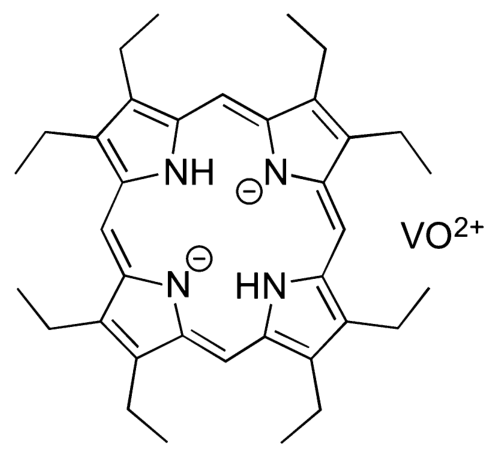
\includegraphics[width=0.85\linewidth]{scheme02_VO_oep.png}\\
    {\scriptsize VO(oep)}
    \column{0.6\textwidth}
    \begin{itemize}
      \item unpaired electron localised on \cgold{vanadium}
      \item<2-> one-electron \emph{oxidation} uses an occupied \cgold{porphyrin} orbital
      \item<3-> one-electron \emph{reduction} uses an unoccupied \cgold{porphyrin} orbital
    \end{itemize}
    \onslide<4->{\small also reported: quantum dots, the LiF dissociation curve}
  \end{columns}
\end{frame}

\begin{frame}{A TEMPO-dithiolate on platinum (Figure 11)}
  \begin{columns}[c]
    \column{0.55\textwidth}
    \centering
    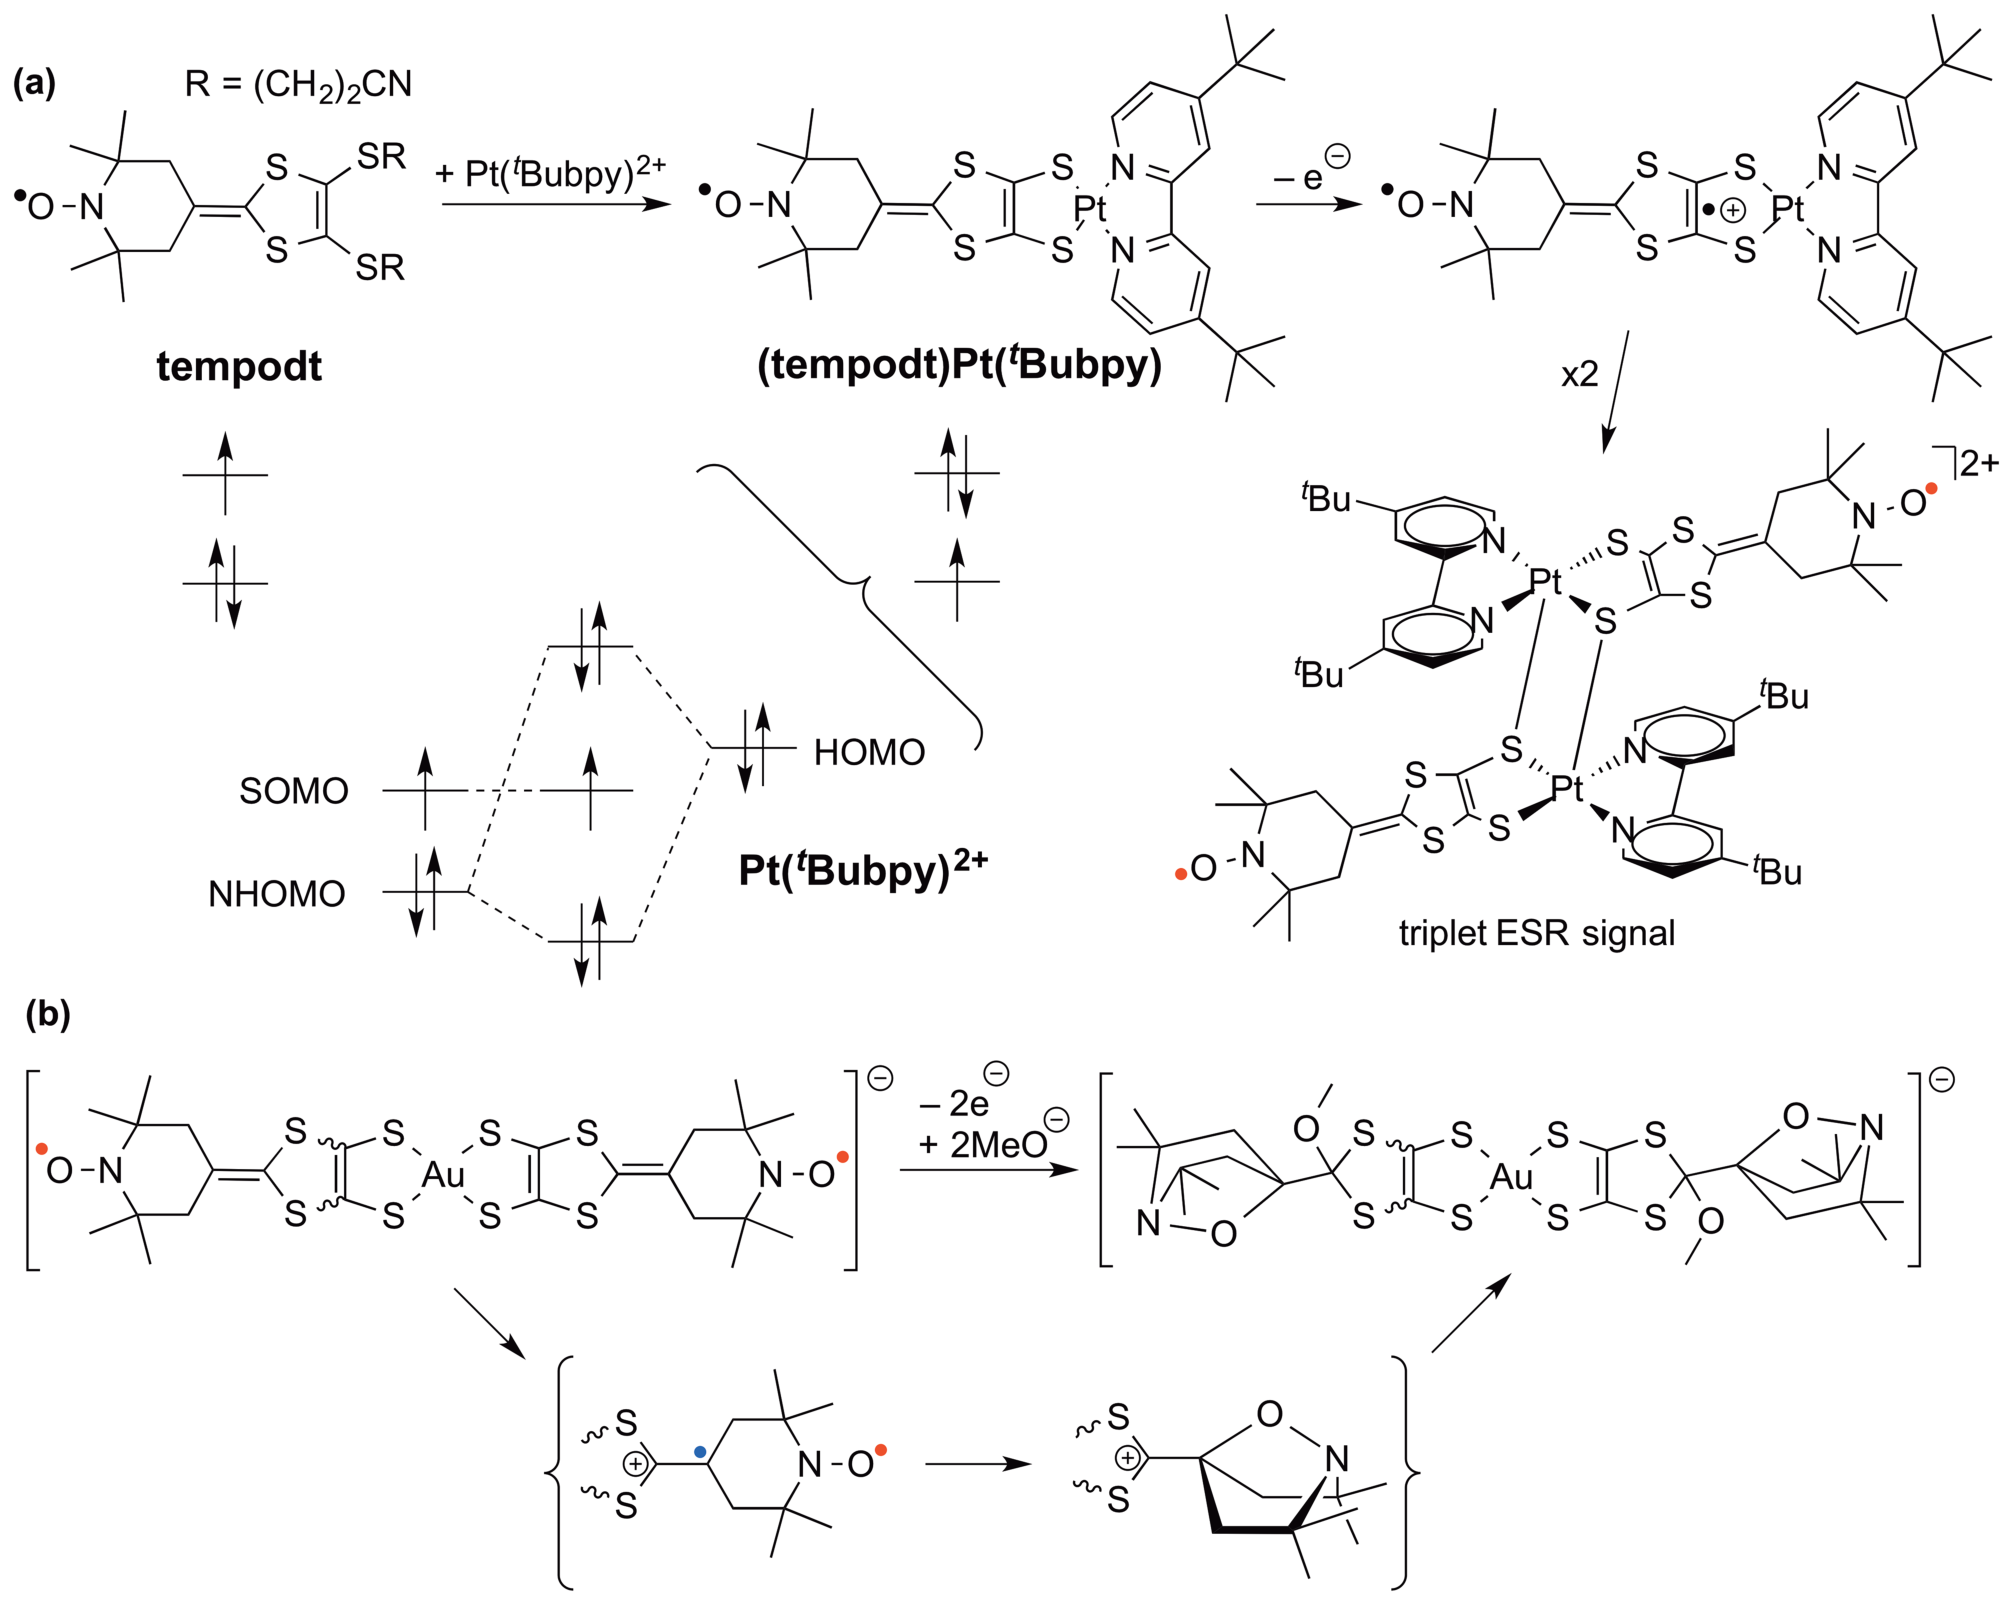
\includegraphics[width=\linewidth]{fig11_tempo_dithiolate_non_aufbau.png}
    \column{0.42\textwidth}
    \small
    \begin{itemize}
      \item oxidation of (tempodt)Pt(tBubpy) removes an electron from the \cgold{dithiolate HOMO}
      \item<2-> evidence: UV--Vis, ESR, CV, DFT and the dimerisation product
      \item<3-> free tempodt is a normal radical; the conversion comes from an antibonding interaction of its NHOMO with the HOMO
        of Pt(tBubpy)$^{2+}$
      \item<4-> (b) a ditempo metalladithiolene: oxidation-generated biradicals couple to a bicyclic product
    \end{itemize}
  \end{columns}
\end{frame}

\begin{frame}{Spin-polarised donors (Figures 12, 13)}
  \begin{columns}[c]
    \column{0.42\textwidth}
    \centering
    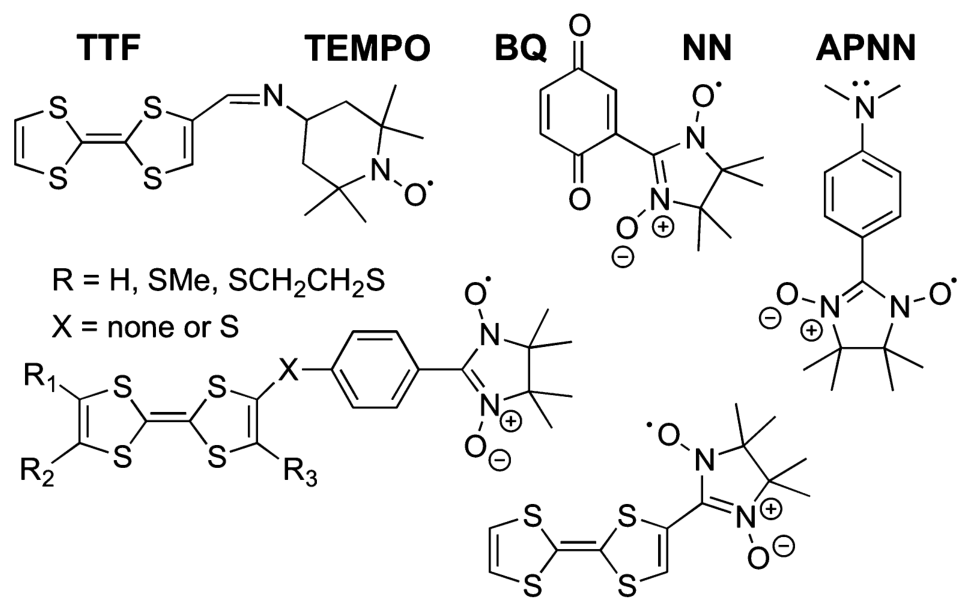
\includegraphics[width=\linewidth]{fig12_nitronyl_nitroxide_donors.png}
    \vskip0.1cm
    \small nitronyl nitroxide (NN) radicals on TTF, BQ, amine donors: one-electron oxidation gives \cgold{triplet cation diradicals}
    \column{0.55\textwidth}
    \onslide<2->{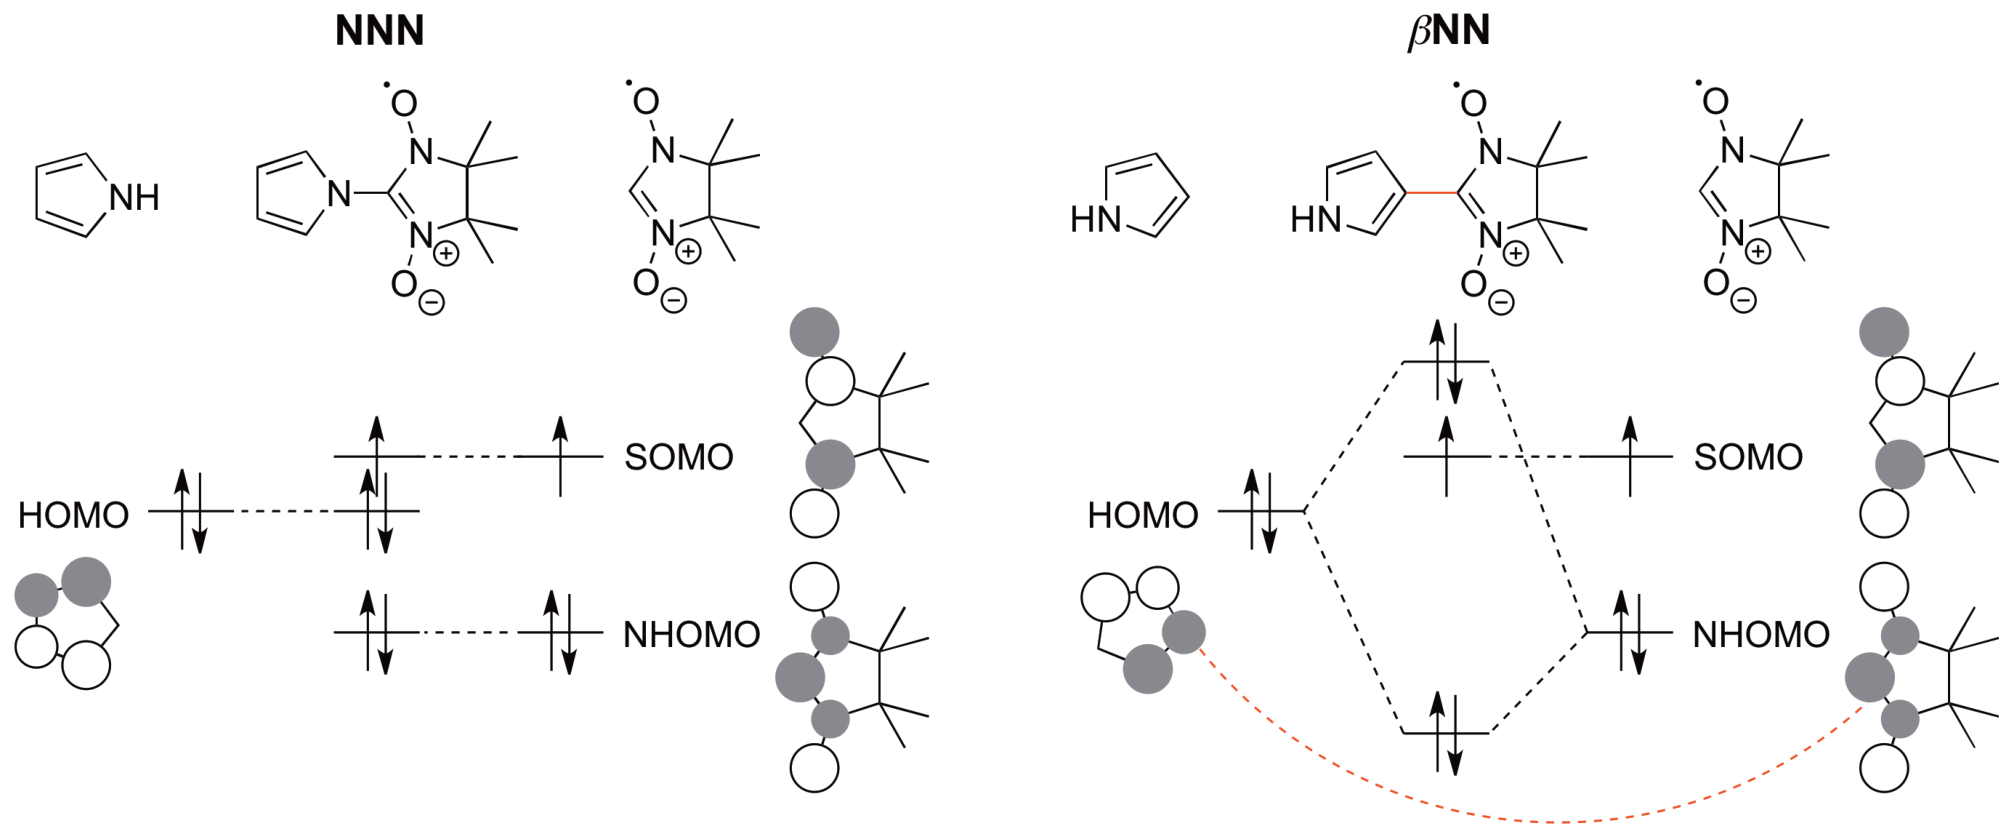
\includegraphics[width=\linewidth]{fig13_disjoint_nondisjoint_orbital_conversion.png}}
    \onslide<3->{\small \cgold{NNN} (1-pyrrolyl): donor HOMO disjoint from SOMO/NHOMO. \cgold{$\beta$NN} (3-pyrrolyl): donor HOMO and NHOMO
      nondisjoint; their combination rises above the SOMO.}
  \end{columns}
\end{frame}

\begin{frame}{Conducting magnets (Scheme 4, Figure 14, Scheme 5)}
  \begin{columns}[c]
    \column{0.5\textwidth}
    \centering
    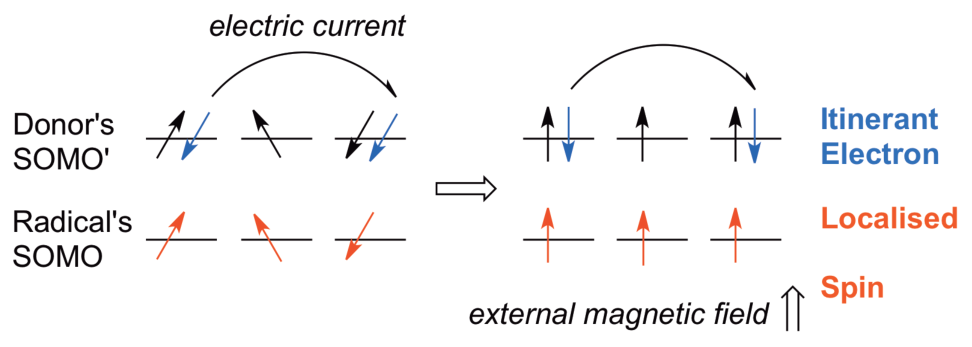
\includegraphics[width=\linewidth]{scheme04_conductivity_magnetism.png}
    \vskip0.1cm
    \only<2-3>{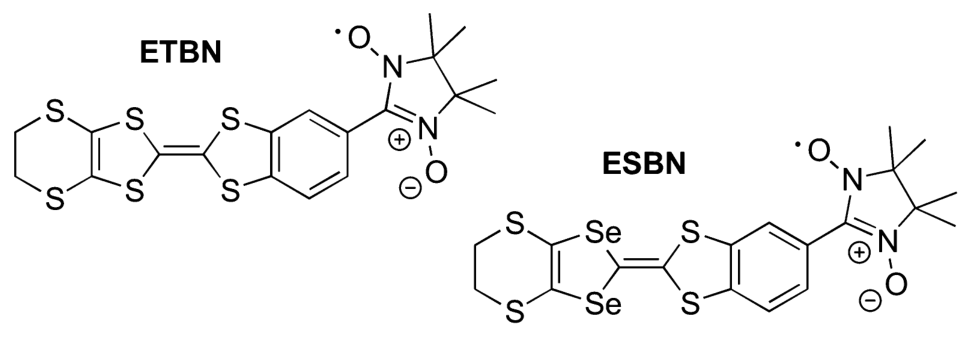
\includegraphics[width=0.8\linewidth]{scheme05_conducting_magnets_ETBN_ESBN.png}}
    \only<4->{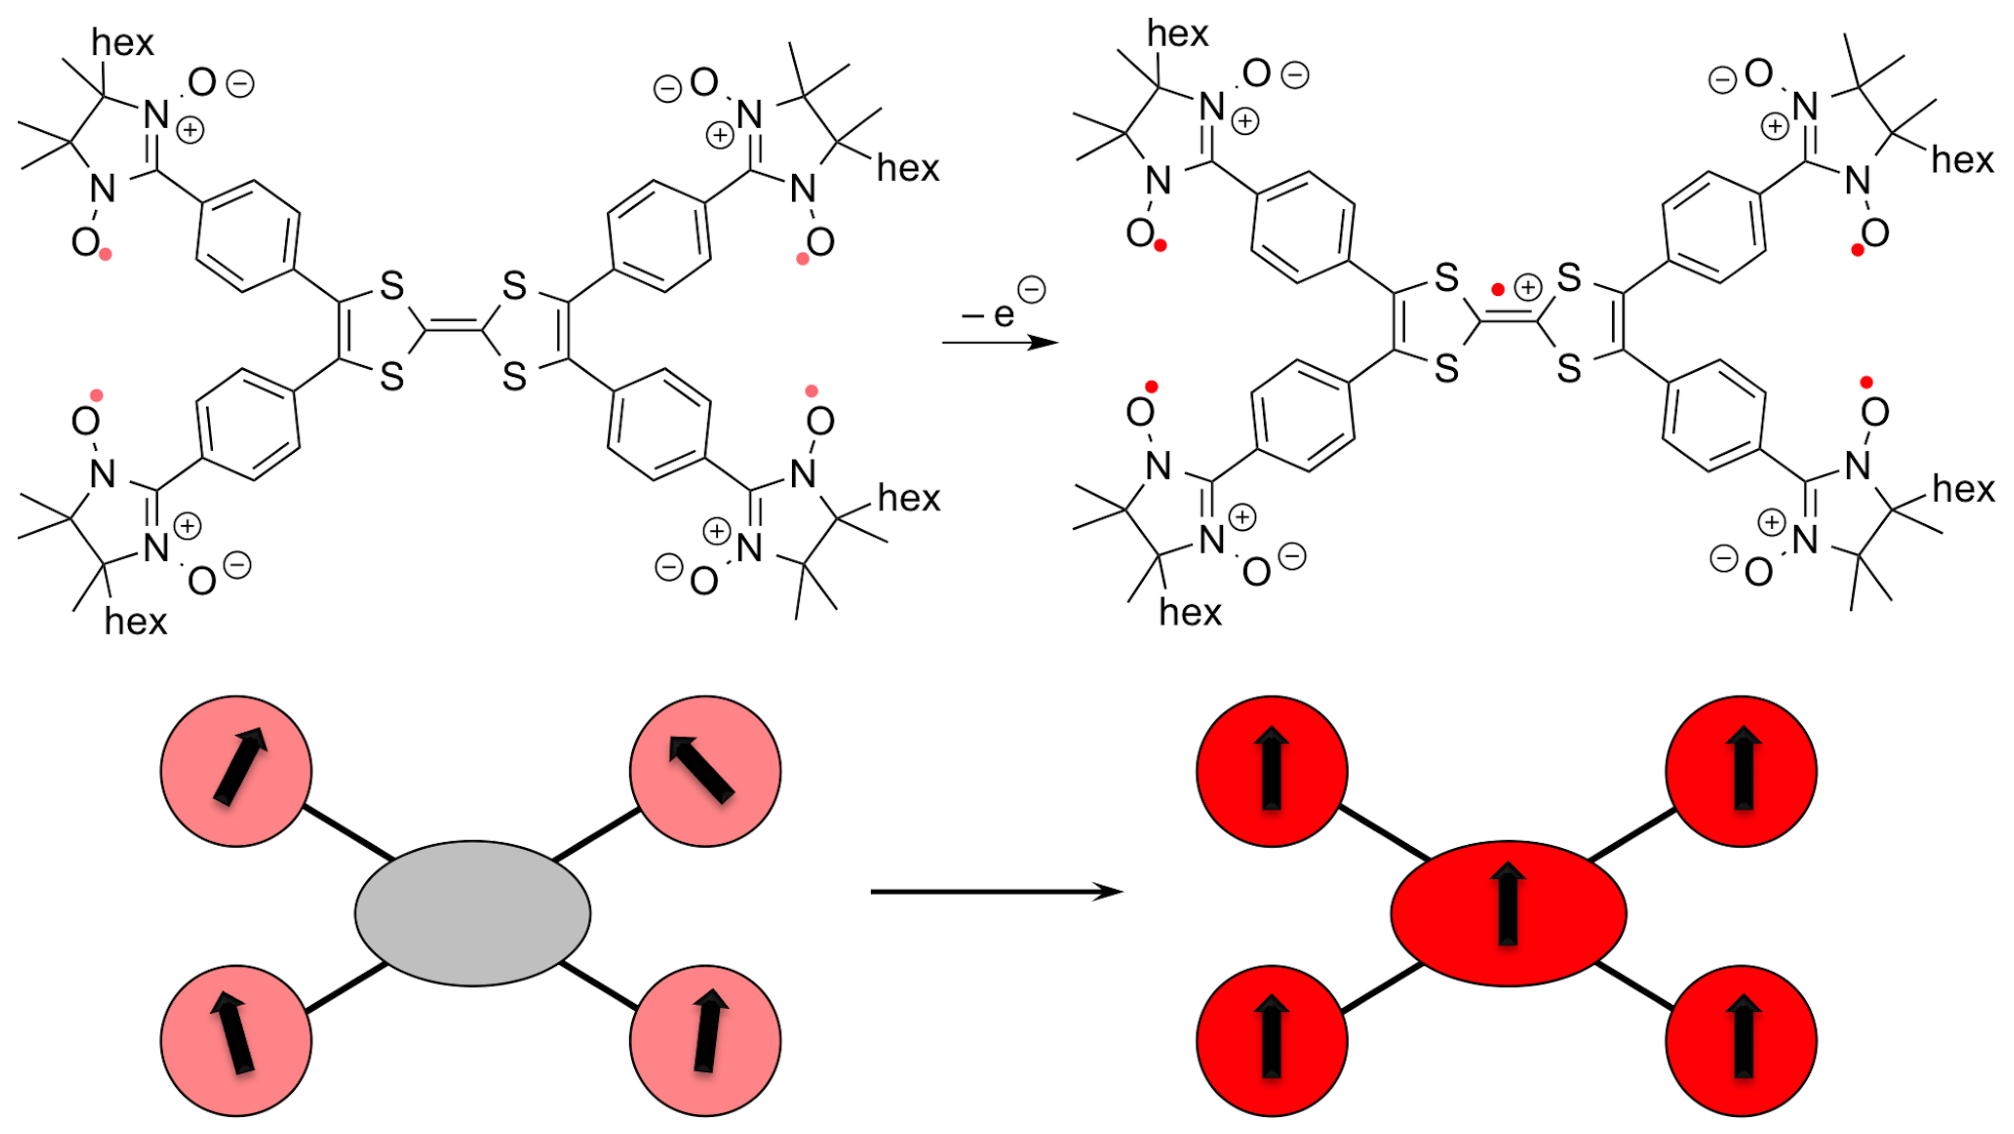
\includegraphics[width=0.95\linewidth]{fig14_oxidation_induced_ferromagnetic_coupling.png}}
    \column{0.47\textwidth}
    \small
    \begin{itemize}
      \item two nondegenerate SOMOs: the donor's (higher) carries an itinerant electron, the radical's (lower) a localised spin
      \item<2-> ETBN, ESBN perchlorate salts: ``first genuine paramagnetic conductors''
      \item<3-> neutral crystals: negative magnetoresistance; field-effect transistors
      \item<4-> Fig.\ 14: several radicals on one donor; oxidation gives a strongly ferromagnetic high-spin system
    \end{itemize}
  \end{columns}
\end{frame}

\begin{frame}{Other radicals, and a pH sensor (Figure 15)}
  \begin{columns}[c]
    \column{0.4\textwidth}
    \centering
    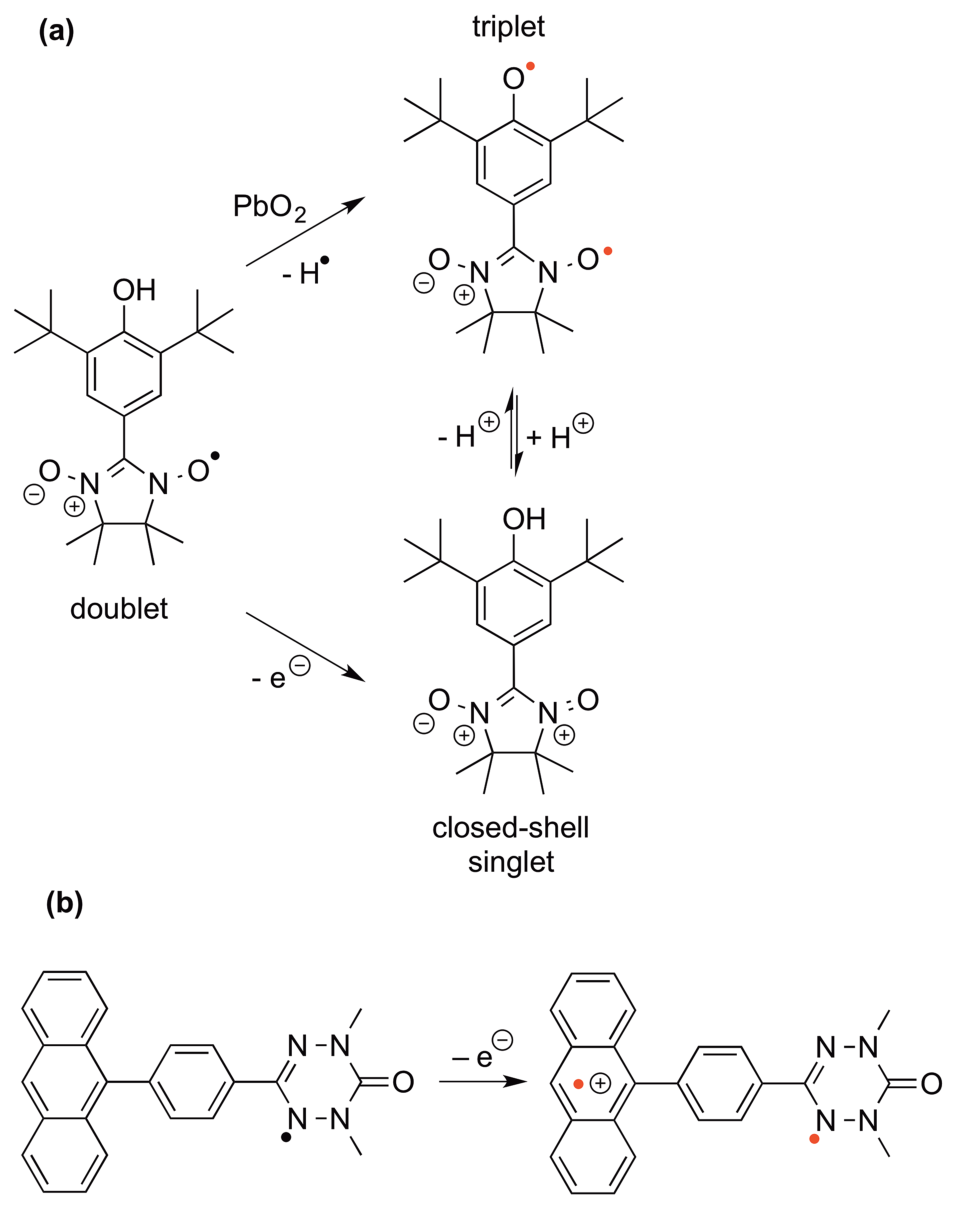
\includegraphics[height=0.66\textheight]{fig15_donors_other_radicals.png}
    \column{0.57\textwidth}
    \begin{itemize}
      \item \cgold{(a)} NN with a phenol-based donor: (de)protonation switches between \emph{triplet} and \emph{closed-shell singlet}:
        a pH sensor
      \item<2-> \cgold{(b)} anthracene--$p$-phenylene--oxoverdazyl (AnOV): high-spin oxidation products
    \end{itemize}
  \end{columns}
\end{frame}

\begin{frame}{Distonic radical anions (Figure 16)}
  \begin{columns}[c]
    \column{0.38\textwidth}
    \centering
    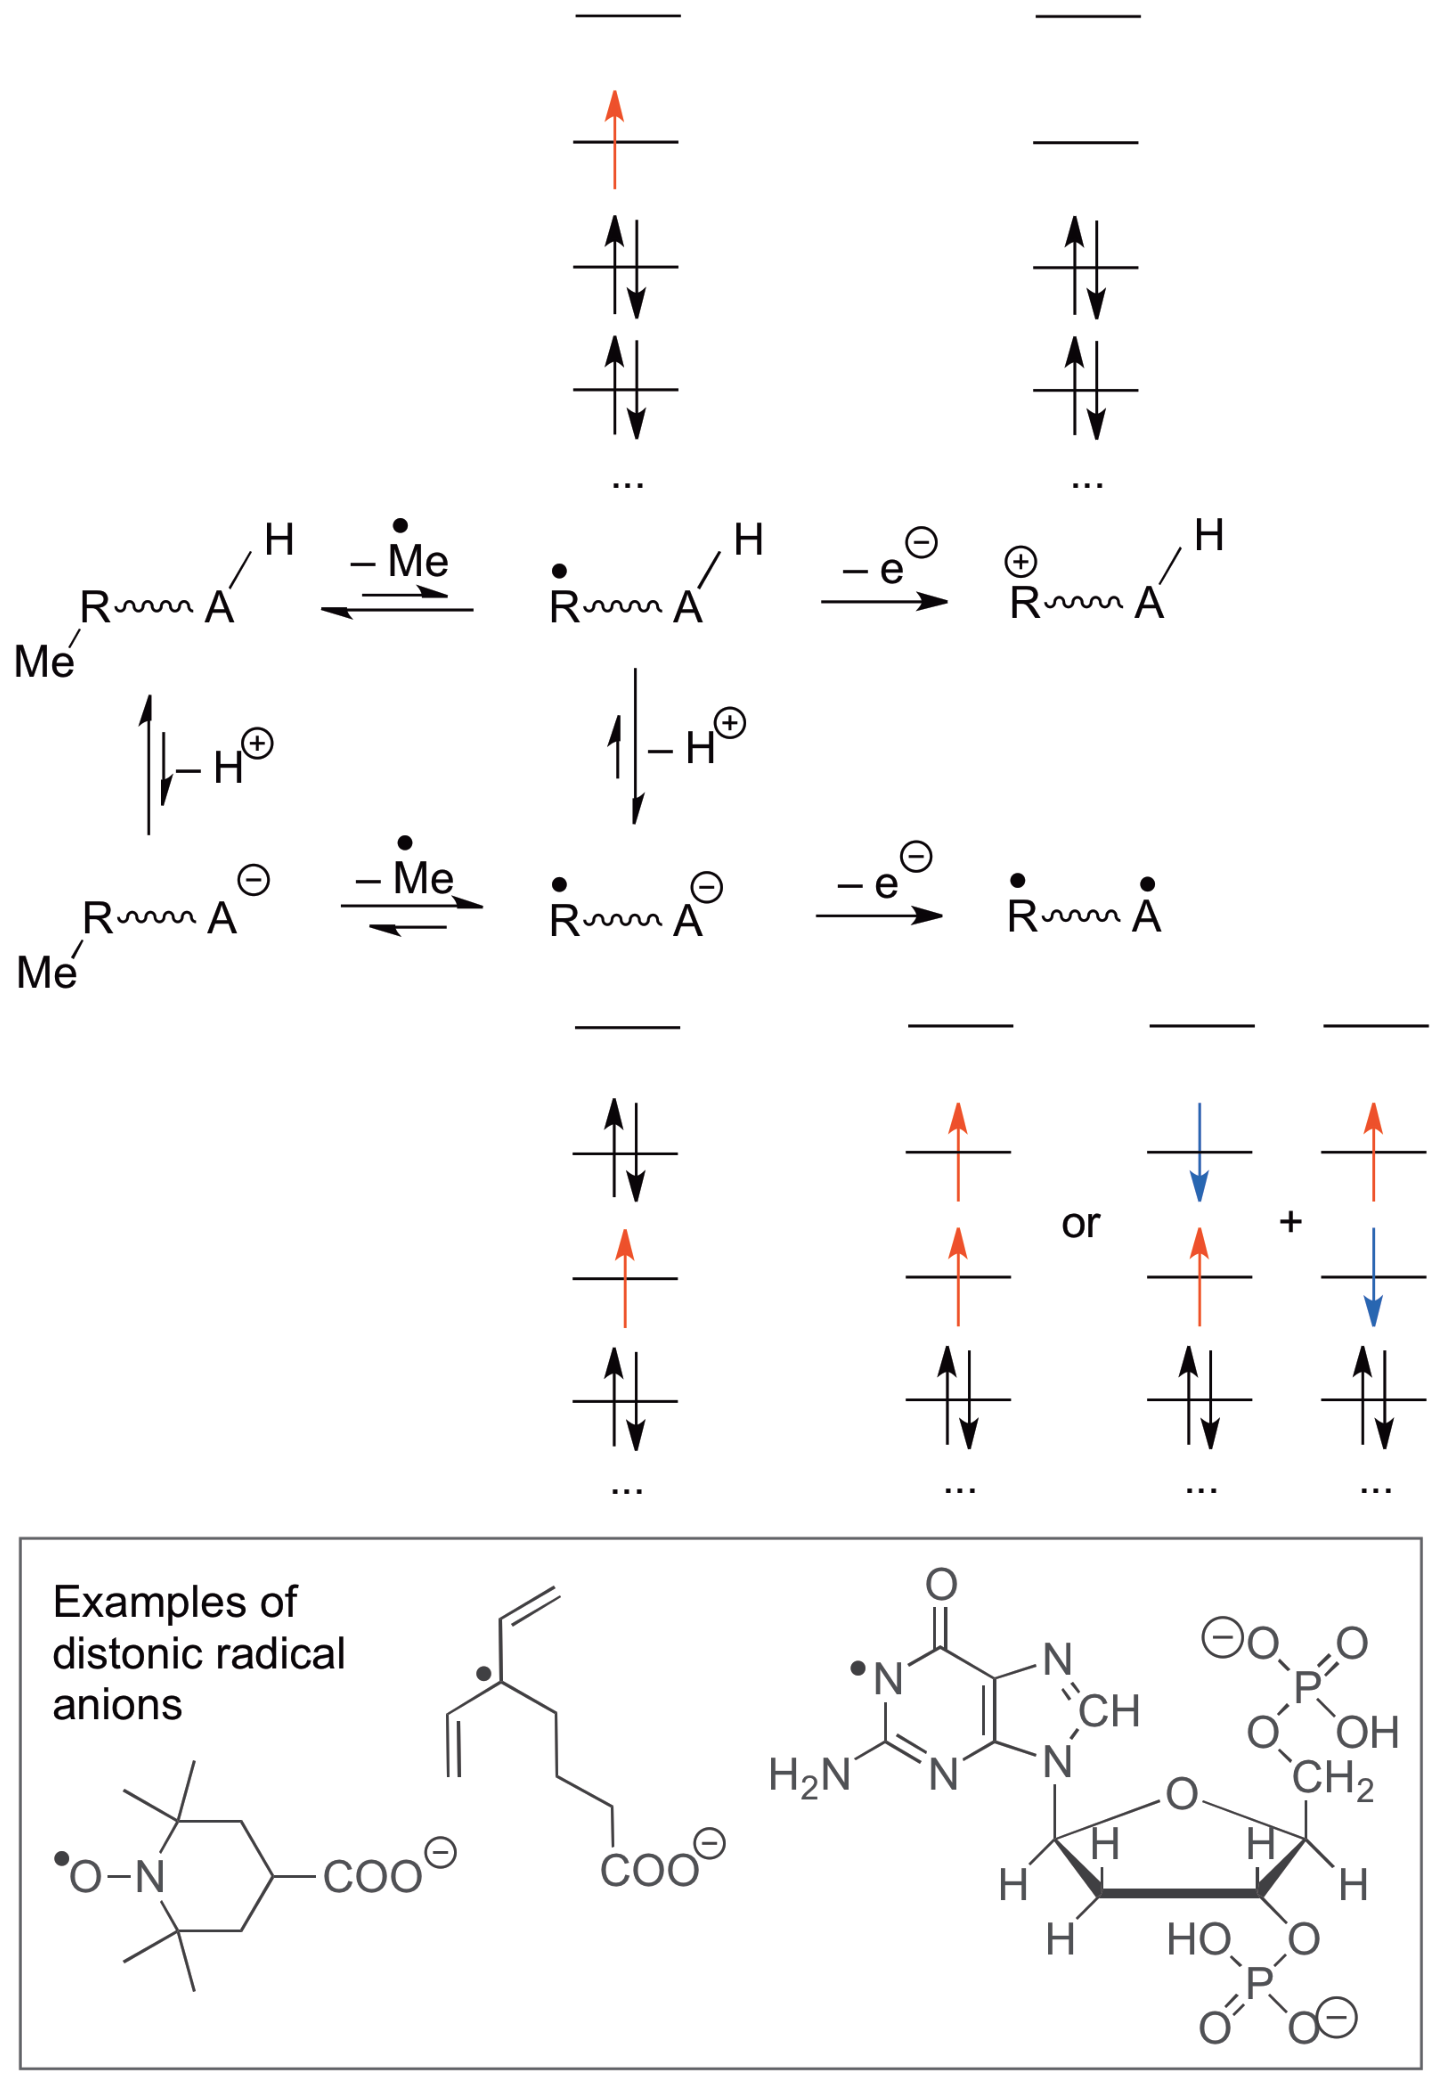
\includegraphics[height=0.78\textheight]{fig16_distonic_radical_anions.png}
    \column{0.59\textwidth}
    \begin{paperclaim}
      a stabilised radical plus an anionic group not $\pi$-conjugated to it: the anion's HOMO lies above the SOMO;
      ``if the anion is protonated, the aufbau orbital occupation is restored'', switchable ``via changing pH''; on oxidation
      the conversion ``yield[s] diradical species preferentially over the closed-shell zwitterion'' (p.\ 452--453)
    \end{paperclaim}
    \onslide<2->{\small \cgold{testable}: compute both oxidised states, with and without the proton}
  \end{columns}
\end{frame}

\begin{frame}{Our test: two radicals, two protonation states, two functionals}{T11/T11c: UB3LYP/6-31G* geometries, vertical oxidation at 6-31+G*}
  \begin{columns}[c]
    \column{0.58\textwidth}
    \begin{tikzpicture}
      \begin{axis}[noirplot,ybar,width=7.8cm,height=5.4cm,bar width=11pt,ymin=-0.6,ymax=1.6,
          symbolic x coords={shortacid,shortanion,tempoacid,tempoanion},xtick=data,
          xticklabels={short acid,short anion,TEMPO acid,TEMPO anion},
          ylabel={$E_T-E_{\text{CS}}$ (eV)},ymajorgrids,legend style={at={(0.5,1.03)},anchor=south,legend columns=2},
          x tick label style={font=\tiny},enlarge x limits=0.18,unbounded coords=discard]
        \addplot[fill=noirgold,draw=none,bar shift=-6pt] table[x=system,y=b3lyp,col sep=comma]{data/distonic.csv};
        \addlegendentry{B3LYP}
        \only<2->{\addplot[fill=noircyan,draw=none,bar shift=6pt] table[x=system,y=camb3lyp,col sep=comma]{data/distonic.csv};}
        \only<2->{\addlegendentry{CAM-B3LYP}}
        \draw[noirfg] (axis cs:shortacid,0) -- (axis cs:tempoanion,0);
      \end{axis}
    \end{tikzpicture}
    \column{0.38\textwidth}
    \small
    $<0$: oxidation gives the \cgreen{diradical}\\
    $>0$: the closed shell
    \begin{itemize}
      \item<1-> acids: closed shell by $1.2$--$1.4$ eV, SOMO $=$ HOMO
      \item<2-> anions, CAM-B3LYP: \cgreen{diradical} by $0.36$ and $0.30$ eV
      \item<3-> anions, B3LYP: misses by $\sim0.07$ eV
    \end{itemize}
  \end{columns}
\end{frame}

\begin{frame}{What the test says}
  \begin{columns}[T]
    \column{0.48\textwidth}
    \cgreen{reproduced}
    \begin{itemize}
      \item SOMO 2--3 levels below the HOMO in the anions; equal to the HOMO in the acids
      \item<2-> protonation moves $E_T-E_{\text{CS}}$ by $\sim1.2$--$1.8$ eV
      \item<3-> with CAM-B3LYP, the anions oxidise to diradicals: \okpill
    \end{itemize}
    \column{0.48\textwidth}
    \onslide<4->{\cgold{caveat}}
    \begin{itemize}
      \item<4-> B3LYP lowers the closed shell by $0.61$ eV vs.\ CAM-B3LYP, the triplet by only $0.17$
      \item<5-> verdict flips at $\sim0.07$ eV: a functional-sensitive claim
      \item<6-> delocalisation error is a plausible cause (not tested)
    \end{itemize}
  \end{columns}
\end{frame}

\begin{frame}{Non-aufbau by electron addition (Figure 17)}
  \begin{columns}[c]
    \column{0.52\textwidth}
    \centering
    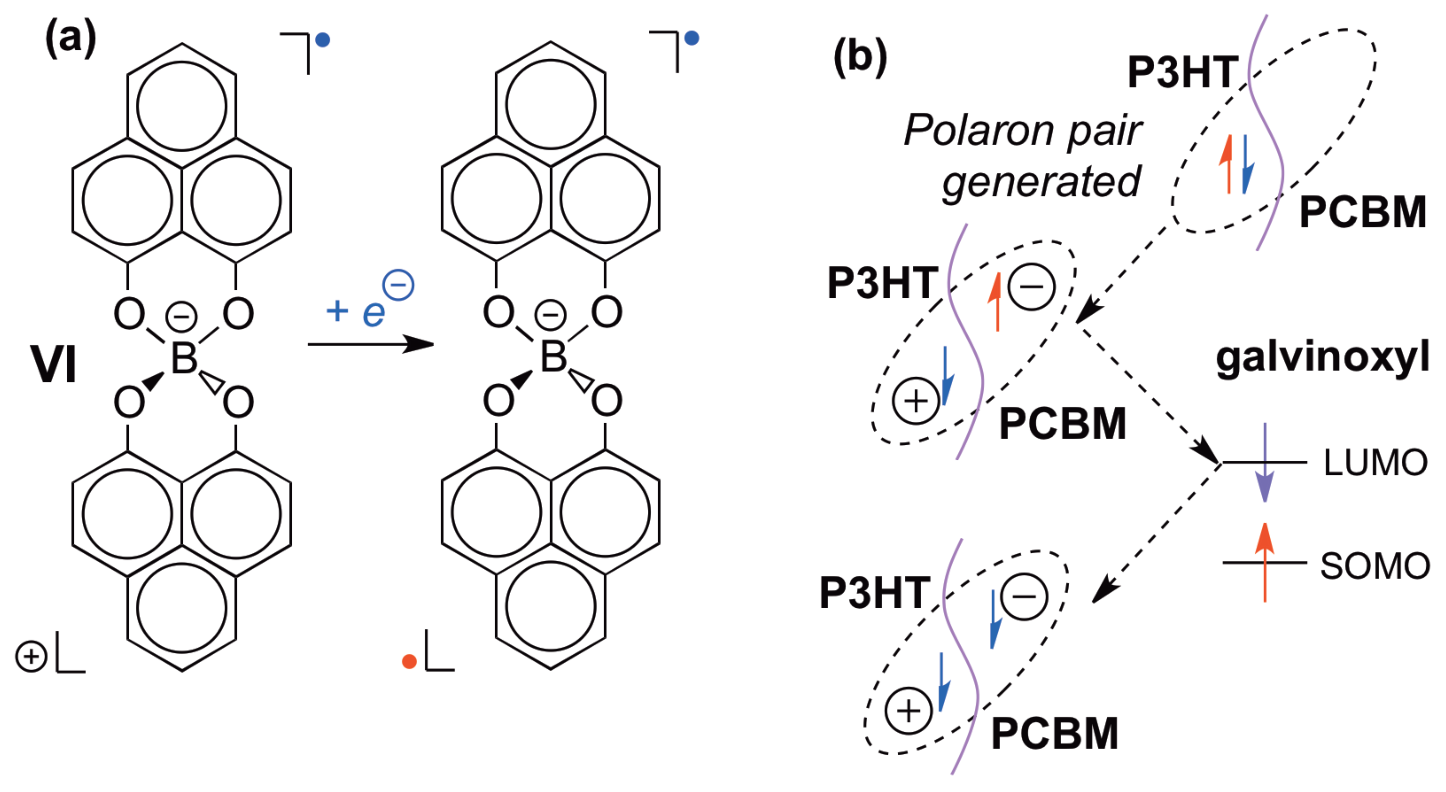
\includegraphics[width=\linewidth]{fig17_non_aufbau_by_electron_addition.png}
    \column{0.45\textwidth}
    \small
    \begin{itemize}
      \item \cgold{(a)} spirobiphenalenyl VI is reduced to an open-shell singlet; it crystallises without dimerising: an intrinsic
        molecular metal
      \item<2-> \cgold{(b)} galvinoxyl in P3HT/PCBM: its LUMO mediates singlet$\to$triplet crossing of polaron pairs via exchange,
        preventing recombination and raising photovoltaic efficiency
      \item<3-> self-doping: in TTFCOO$^-$NH$_4^+$ the SOMO of TTF$^{+\bullet}$ is not the highest occupied orbital
    \end{itemize}
  \end{columns}
\end{frame}
